In this section we present a method to derive concurrency oracles from the instruction
semantics encoded in the  metalanguage (Definition~\ref{def:metalanguage}).
More specifically, we aim to reason about instructions that
have only \emph{static dependencies}.

We start by introducing formal definitions and Haskell encodings of the concepts
required for building concurrency oracles.
First, we define the notions of input and output dependencies of a computation.

\textbf{Definition (input dependency):\label{def:in-dependencies}}
Consider a term $f$ of an applicative metalanguage~\hs{Semantics Applicative a}.
A key $k$ is an~\emph{input dependency} of the term $f$ if the term $f$
performs a~\hs{read} of the key $k$.

\textbf{Definition (output dependency):\label{def:out-dependencies}}
Consider a term $f$ of an applicative metalanguage~\hs{Semantics Applicative a}.
A key $k$ is an~\emph{output dependency} of the term $f$ if the term $f$
performs a~\hs{write} of the key $k$.

\textbf{Definition (dependencies):\label{def:dependencies}}
Consider a term $f$ of an applicative metalanguage~\hs{Semantics Applicative a}.
The~\emph{dependencies} of the term $f$ are a pair of sets $I$ and $O$,
comprising the input and output dependencies of the term $f$, respectively.

In the Haskell implementation, we do not distinguish between input and output dependencies
in the type level, thus the function determining the dependencies of a computation
has the following type:

\begin{minted}[xleftmargin=10pt]{haskell}
dependencies :: Semantics Applicative a -> Maybe ([Key], [Key])
\end{minted}

\noindent
The~\hs{Maybe} type constructor comes from the definition of the metalanguage:
if the applicative semantics is partial (returns~\hs{Nothing}) it is impossible
to extract its static dependencies. Successful static analysis yields a pair of
lists representing the sets of input and output dependencies of a computation.

To extract the static data dependencies of an applicative computation we need to
interpret its semantics in the special context of a \emph{constant functor}.

\subsection{The constant functor}

The~\hs{Const a b} data type is defined as follows~\cite{Mcbride:2008:APE:1348940.1348941}:

\begin{minted}[xleftmargin=10pt]{haskell}
newtype Const a b = Const { getConst :: a }
\end{minted}

\noindent
A value of the~\hs{Const a b} is just a value of any type~\hs{a}
wrapped in a data constructor. However, it is important that the type constructor
has a~\emph{phantom type} variable. This type variable allows us to
declare useful instances of standard Haskell type classes such as~\hs{Functor}
and \hs{Applicative} for \hs{Const a}. We would like to use this data type as a
computational context for applicative semantics, hence we declare the
corresponding instance\footnote{\hs{Const a} also has a \hs{Functor} instance,
where~\hs{fmap _ (Const x) = Const x}}:

\begin{minted}[xleftmargin=10pt]{haskell}
instance Monoid m => Applicative (Const m) where
    pure _              = Const mempty
    Const x <*> Const y = Const (x `mappend` y)
\end{minted}

This instance exactly describes the desired behaviour of static dependency tracking
computational context.~\hs{Const [Key]} is an applicative functor that ignores
its enclosed value, but accumulates the declared dependencies using the~\hs{Monoid}
instance for Haskell list data type\footnote{The empty list~\hs{[]} is the
neutral element and the list concatenation~\hs{(++)} is the associative binary operation}.

\subsection{Extracting dependencies}

Using the elegant~\hs{Const a b} abstraction we define the \hs{dependencies} function:

\begin{minted}[xleftmargin=10pt]{haskell}
dependencies :: Semantics Applicative a -> Maybe ([Key], [Key])
dependencies s = partitionEithers . getConst <$> s read write
  where read  k    =       Const [Left  k]
        write k fv = fv *> Const [Right k]
\end{minted}

\noindent
We instantiate the polymorphic computation context with \hs{f = Const [Key]}
and supply custom tracking \hs{read} and \hs{write} functions. In fact, \hs{read}
does not perform any reading and just tracks the key as an input dependency,
whereas \hs{write} tracks the key as an output dependency and executes the
effectful computation \hs{fv}, to appropriately track its dependencies. The
resulting list of keys gets unwrapped and unzipped by
\hs{partitionEithers}~\hs{.}~\hs{getConst}.

Now we are fully armed to define concurrency oracles for terms of the
applicative metalanguage.

\subsection{Concurrency oracle}
% \vspace{-2em}
A concurrency oracle is a function taking two computations and statically
determining if they are data~\emph{concurrent}, i.e. do not share any
data dependencies.


\textbf{Definition (Concurrency Oracle Answer):\label{def:concurrency-status}}
Two terms of the metalanguage are \emph{concurrent} if they do not share any
data dependencies. They are in a \emph{read} or \emph{write conflict} if they
share any input or output dependencies, respectively. If the share both input
and output dependencies then they are considered to be in a \emph{read-write
conflict}. We use the following data type is used to encode concurrency oracle
answers:

\begin{minted}[xleftmargin=10pt]{haskell}
data OracleAnswer k = Concurrent
                    | ReadConflict [k]
                    | WriteConflict [k]
                    | ReadWriteConflict [k]
\end{minted}

\textbf{Definition (concurrency oracle):\label{def:oracle}}
Consider two terms with applicative semantics $s1$ and $s2$ of
type~\hs{Semantics Applicative a}. A~\emph{concurrency oracle} is defined as the
Haskell function:
% \vspace{-3em}
\begin{minted}[xleftmargin=10pt]{haskell}
concurrencyOracle :: Eq k => Semantics Applicative k v1 a
                          -> Semantics Applicative k v2 a
                          -> Maybe (OracleAnswer k)
concurrencyOracle s1 s2 = do
    (r1, w1) <- dependencies s1
    (r2, w2) <- dependencies s2
    let readConflicts      = intersect r1 r2
        writeConflicts     = intersect w1 w2
        readWriteConflicts = intersect (r1 ++ w1) (r2 ++ w2)
    pure $ case (readConflicts, writeConflicts, readWriteConflicts) of
        ([], [], [] ) -> Concurrent
        (rs, [], rws) | rs == rws -> ReadConflict rs
        ([], ws, rws) | ws == rws -> WriteConflict ws
        (_ , _ , rws) -> ReadWriteConflict rws
\end{minted}
% \vspace{-3em}

The oracle determines static dependencies of two given terms and examines
several possible cases of the intersections of their input and output
dependencies.

\subsection{Example oracles}

In this subsection we show two examples to illustrate the usage of concurrency
oracles. The examples are given in the form of interactive sessions, where
`\hs{ghci>}' denotes the command prompt.

Two \hs{Load} instructions with different arguments are concurrent as confirmed
by the oracle returning the result \hs{Just Concurrent}:

\begin{minted}[xleftmargin=10pt]{haskell}
ghci> concurrencyOracle (semanticsA (Load R0 0))
                        (semanticsA (Load R1 1))
Just Concurrent
\end{minted}

\noindent
Extending the first computation with an additional \hs{Add} instruction causes
a read conflict:
\begin{minted}[xleftmargin=10pt]{haskell}
ghci> let p1 = blockSemanticsA [ Load R0 0
                               , Add  R0 1 ]
ghci> let p2 = semanticsA (Load R1 1))
ghci> concurrencyOracle
Just (ReadConflict [Addr 1])
\end{minted}
We can produce a graphical representation of dependencies between and
within programs \hs{p1} and \hs{p2} with the following commands:

\begin{minted}[xleftmargin=10pt]{haskell}
ghci> let g1 = programDataGraph (zip [0..] [Load R0 0, Add R0 1])
ghci> let g2 = programDataGraph (zip [0..] [Load R1 1])
ghci> drawGraph (overlay g1 g2)
\end{minted}

The resulting dependency graph is shown in Fig.~\ref{fig-example-graph}.
% In the graph, instructions labelled with 1 and 2 belong to the blocks~\hs{p1}
% and~\hs{p2} respectively.
As one can see, both computations share the register \hs{R0}, just like the
oracle has determined.

\begin{figure}
\vspace{-4mm}
\centerline{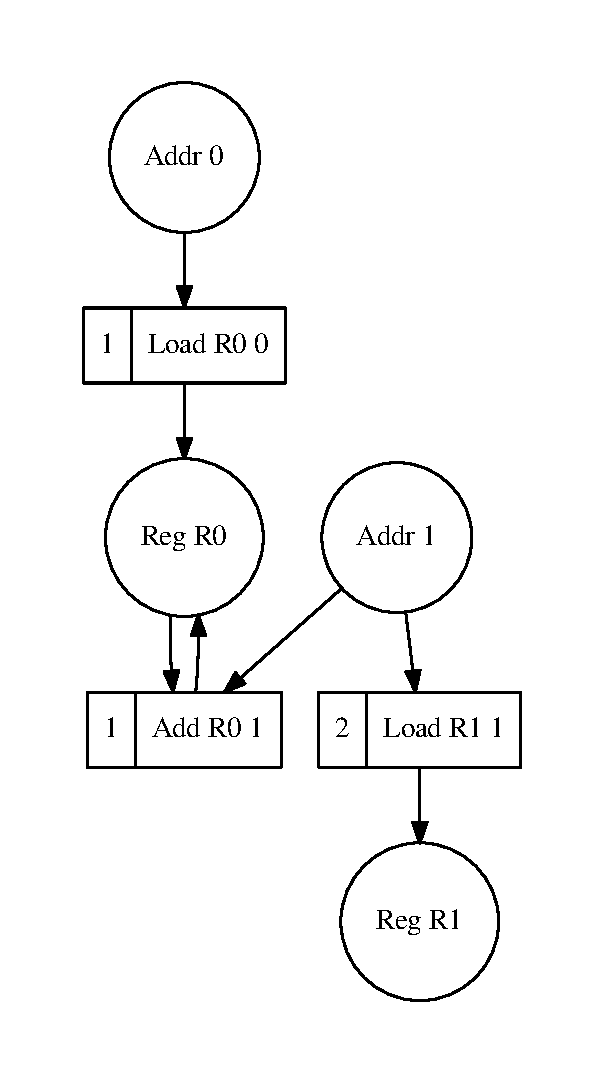
\includegraphics[scale=0.7]{img/oracle2.pdf}}
\vspace{-4mm}
\caption{An overlay of static dependency graphs of two blocks of instructions.\label{fig-example-graph}}
\vspace{-4mm}
\end{figure}
